

\setcounter{section}{0}
%==========================================

\setcounter{figure}{0}
\setcounter{table}{0}
\setcounter{equation}{0}

\chapter{结果讨论}
% To add a non-numbered chapter
%\addcontentsline{toc}{第一章}{相对论重离子碰撞}
% To insert this section on the table of contents

在前文中提到,在本分析当中感兴趣的主要是受介质影响的$\rho$介子质量谱和来自于夸克胶子等离子体热辐射的双电子。这两部分的产额并没有添加到强子衰变模拟当中,这就意味着如果从数据中扣除强子衰变模拟的结果。所剩下的即为我们感兴趣的不便质量谱——双电子额外产额谱。

图\ref{fig:Hm_fullCorr_vsCKTs_54GeV_icent0}为0-80\%中心度下经过效率修正和探测器接收度修正后的双电子谱和经过探测器接收度修正强子衰变模拟结果比较。可以很明显地看到,在低质量区间和中等质量区间数据点要高于强子衰变模拟的结果。这就意味着相比于STAR之前的双电子谱测量,\sNN = 54.4 GeV的测量是一个很好的研究来源于夸克胶子等离子体热辐射的双电子谱的机会。并且在STAR的束流能量扫描二阶段(Beam Energy Scan Phase II, BES-II)项目当中,STAR于2019年取了高统计量的\sNN = 27 GeV金-金对撞的数据。因为其与本分析当中的束流对撞质心能量接近,在最后的讨论中\sNN = 27 GeV的结果会和\sNN = 54.4 GeV的结果一起进行讨论。在接下来的几个小节当中将会对不同的物理区间当中的结果分别进行讨论。

\begin{figure}[htb]
    \begin{center}
    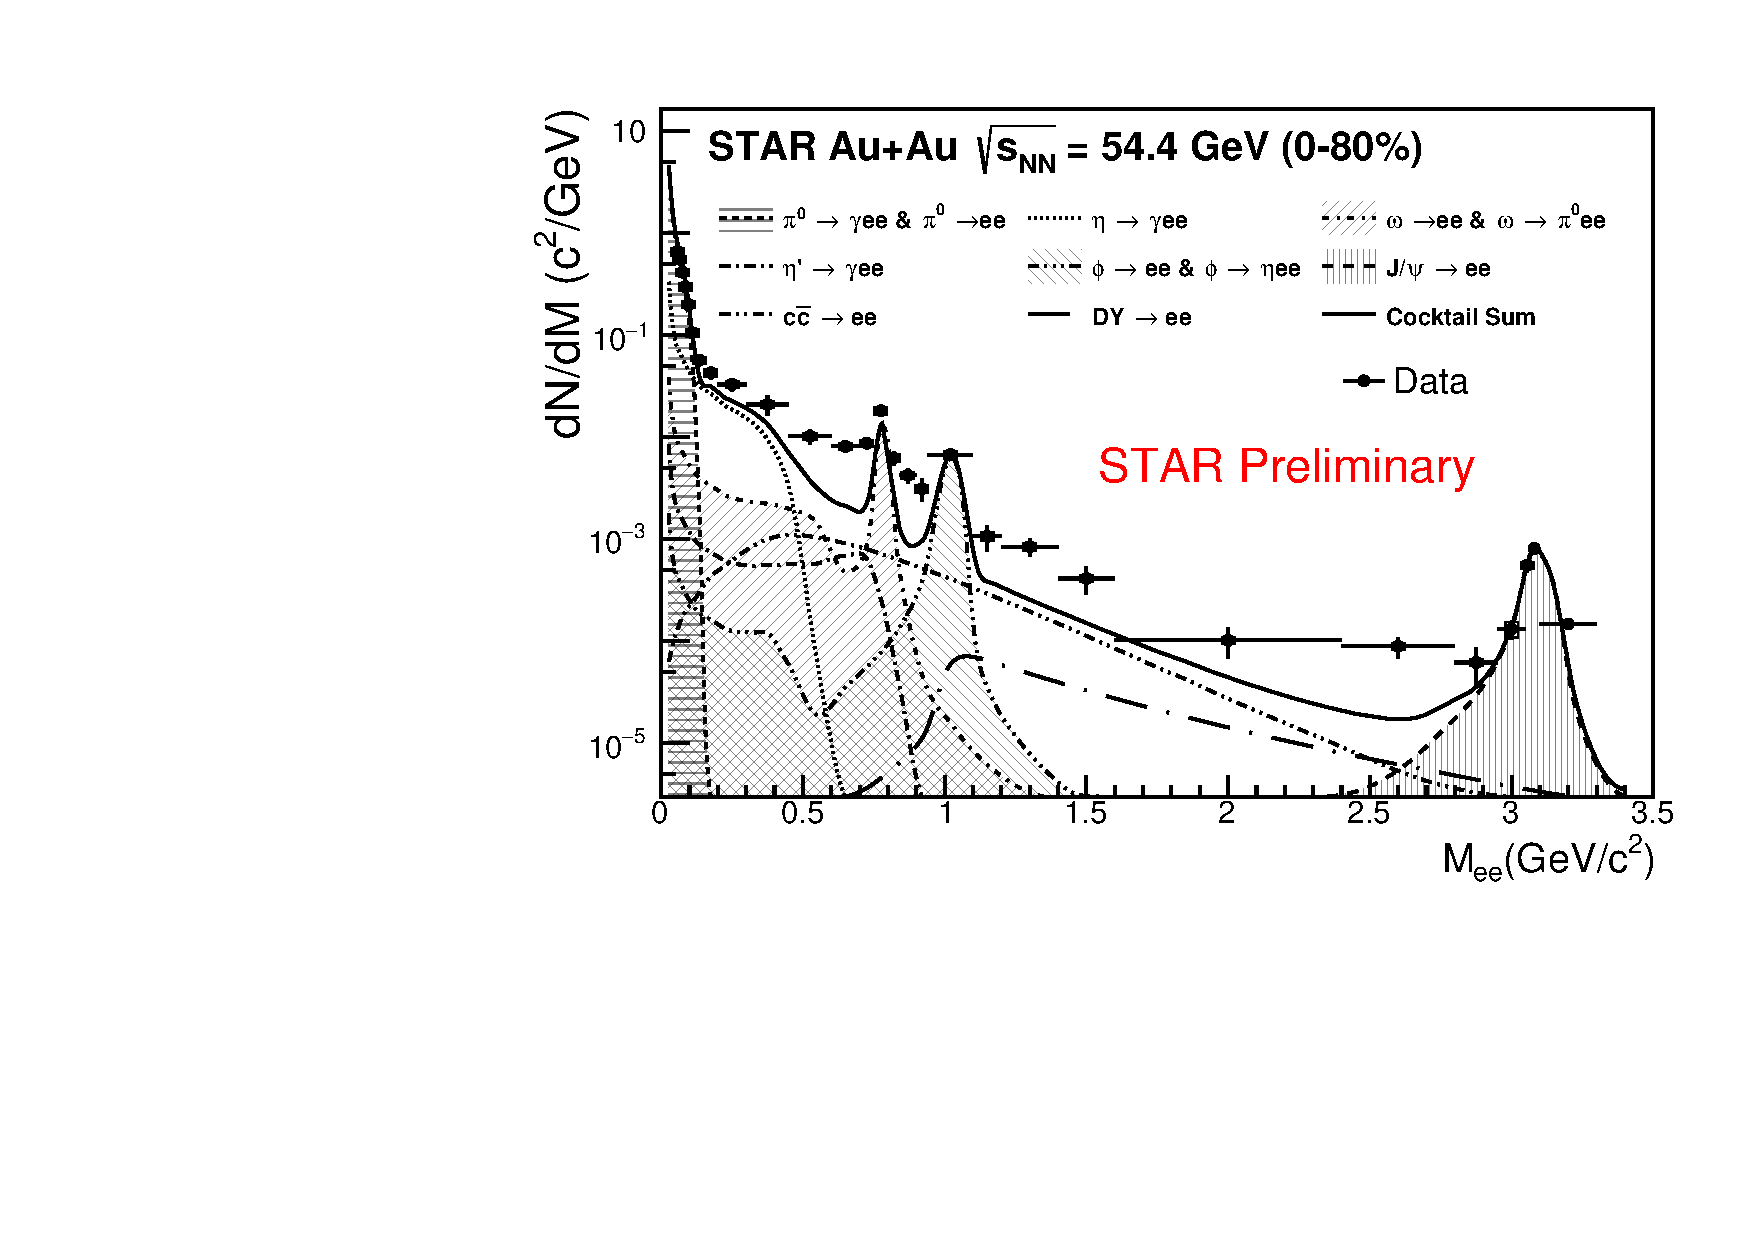
\includegraphics[width=0.75\textwidth,clip]{figures/Chapter4/Hm_fullCorr_vsCKTs_54GeV_icent0.pdf}
    \end{center}
    \caption[\sNN = 54.4 GeV金-金对撞当中0-80\%中心度下双电子谱和强子衰变模拟结果比较]{\sNN = 54.4 GeV金-金对撞当中0-80\%中心度下双电子谱和强子衰变模拟结果比较,强子衰变模拟的不同分量在图中用不同形式的线和填充进行标记}
    \label{fig:Hm_fullCorr_vsCKTs_54GeV_icent0}
\end{figure}

% 在得到双轻子额外产额谱之后,我们可以通过拟合的方法来获取系统的温度。本分析中用了不同的拟合方法来对温度进行抽取。拟合方程分别为 (a)$f(M_{ll}) = (a*BW+b*M^{3/2})*e^{-M/T}$和(b)$f(M_{ll}) = b*M^{3/2}*e^{-m/T}$。不同的拟合方法的到的结果物理意义也不尽相同,具体情况会在本章节中进行讨论。所有的拟合结果如图\ref{fig:Excess_fit}所示,拟合得到的温度参数被列在表\ref{tab:T_fitting_result}当中。

% \begin{figure}[htb]
%     \begin{center}
%     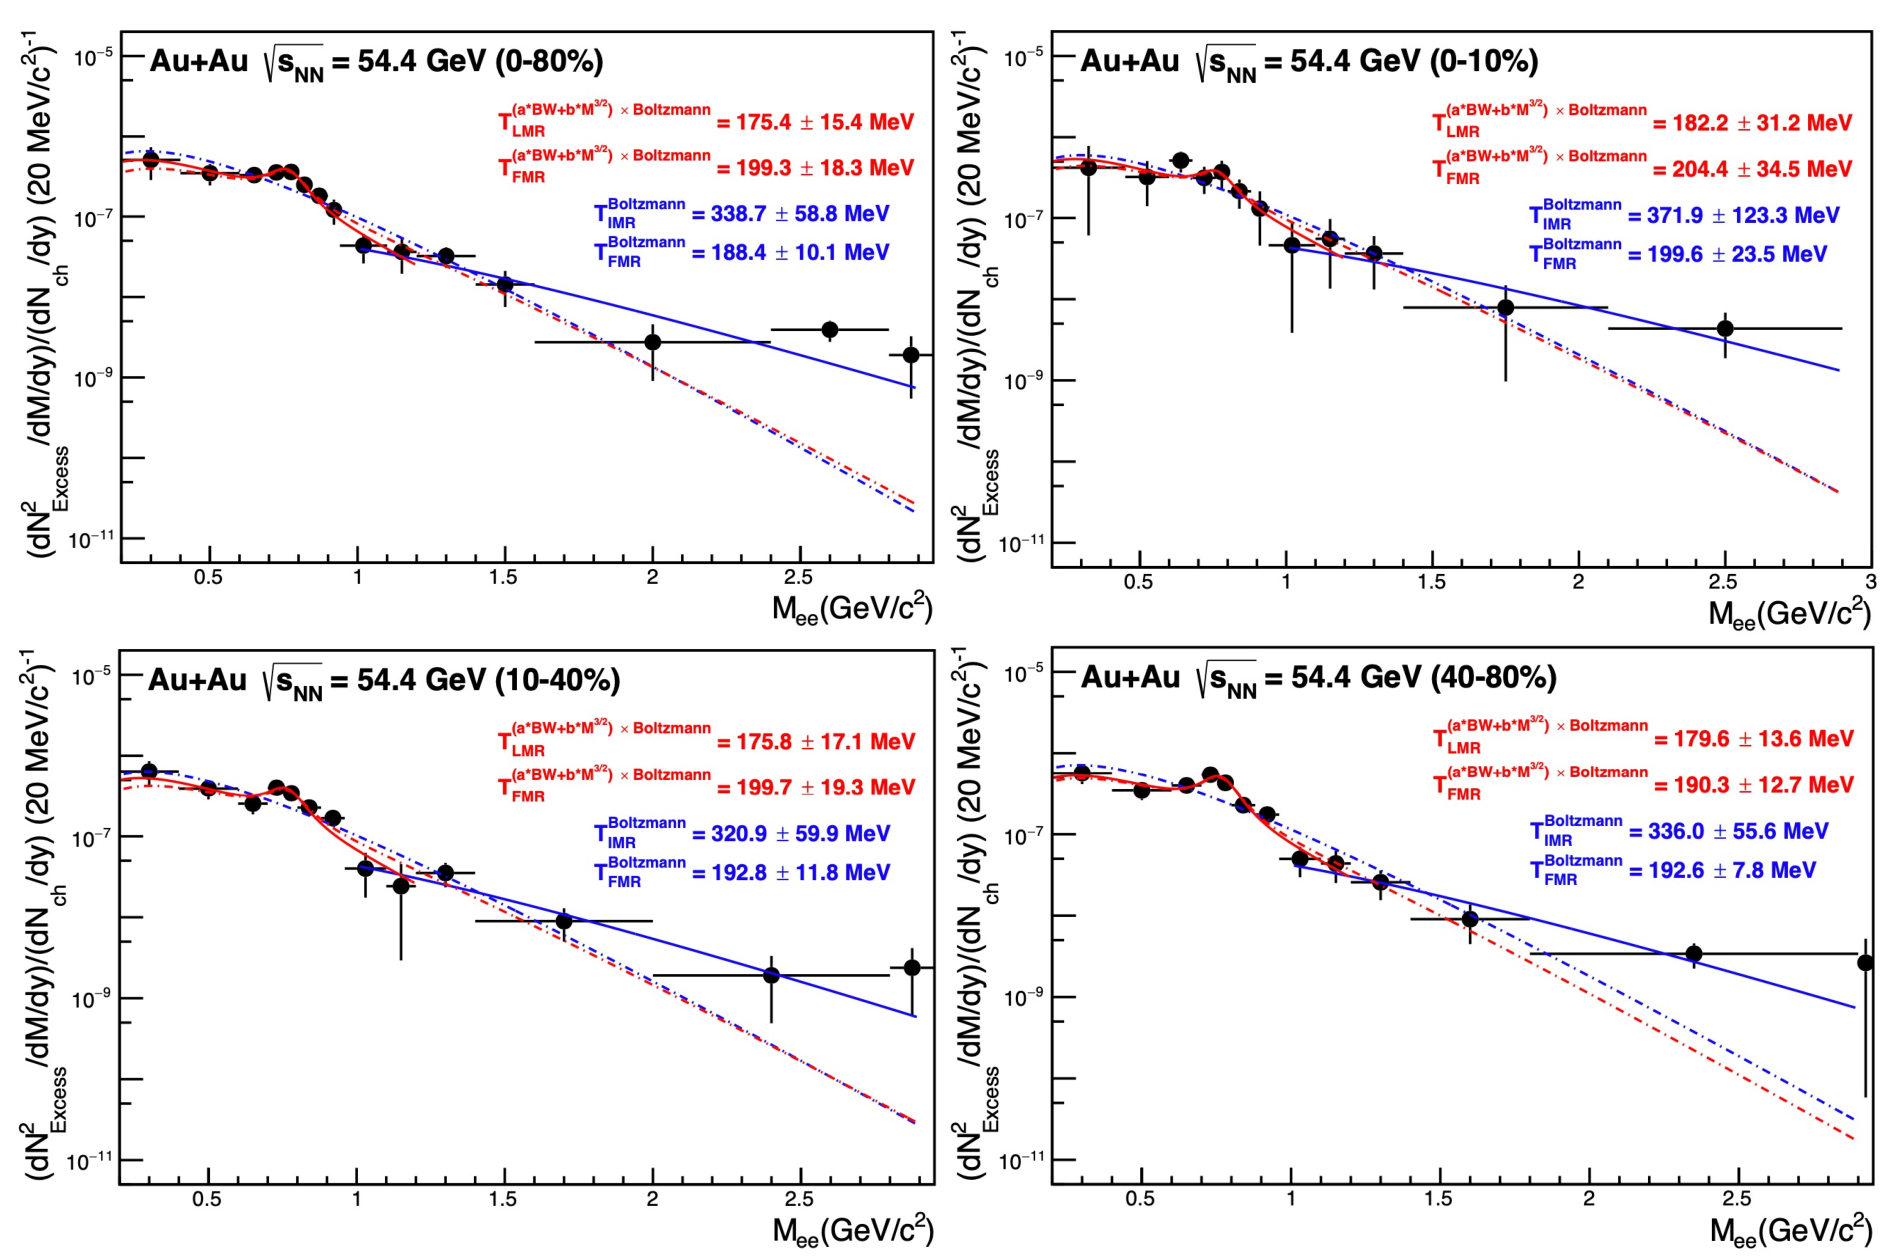
\includegraphics[width=0.75\textwidth,clip]{figures/Chapter4/Excess_fit.pdf}
%     \end{center}
%     \caption[\sNN = 54.4 GeV金-金对撞当中不同中心度下双电子额外产额谱及拟合结果示意图]{\sNN = 54.4 GeV金-金对撞当中不同中心度下双电子额外产额谱及拟合结果示意图,采用的拟合区间和拟合方程在图中进行标示,方程的具体形式见式\ref{}和\ref{}}
%     \label{fig:Excess_fit}
% \end{figure}

% \begin{table}[h!]
%     \centering
%     \caption{54.4GeV金-金对撞中不同中心度下不同拟合方式抽取得到的温度的值}
%     \label{tab:T_fitting_result}
%     \begin{tabularx}{1\textwidth} {
%     | >{\centering\arraybackslash}X |>{\centering\arraybackslash}X |>{\centering\arraybackslash}X |>{\centering\arraybackslash}X |>{\centering\arraybackslash}X | }
%         \hline
%         Centrality & fit function : (a), LMR  & fit function : (a), FMR & fit function : (b), IMR & fit function : (b), FMR   \\
%         \hline
%         0-80\%  & $175.4 \pm 15.4$ & $199.3 \pm 18.3$ & $338.7 \pm 58.8$ & $188.4 \pm 10.1$  \\
%         \hline
%         0-10\%  & $182.2 \pm 31.2$ & $204.4 \pm 34.5$ & $371.9 \pm 123.3$ & $199.6 \pm 23.5$ \\
%         \hline
%         10-40\% & $175.8 \pm 17.1$ & $199.7 \pm 19.3$ & $320.9 \pm 59.9$ & $192.8 \pm 11.8$ \\
%         \hline
%         40-80\% & $197.6 \pm 13.6$ & $190.3 \pm 12.7$ & $336.0 \pm 55.6$ & $192.6 \pm 7.8$ \\
%         \hline
%     \end{tabularx}
% \end{table}

\subsection{低质量区间}


\section{中等质量区间}

在中等质量区间当中,夸克胶子等离子体热辐射所产生的双电子占据了主要部分。所以在这个质量区间的拟合当中只使用了\ref{eq:QGP_thermal}作为拟合方程。NA60实验也在\sNN = 17.3 GeV铟-铟对撞中对来源于夸克胶子等离子体热辐射的双轻子进行了测量,其测量得到的温度结果为205 $\rm{ \pm }$ 12 MeV\cite{Specht:2010xu}。STAR实验\sNN = 54.4 GeV, \sNN = 27 GeV 金-金对撞中在双电子谱的中等质量区间抽取结果如图\ref{fig:Hm_ExY_FMR_54GeV_27GeV_NA60_QGPfit_icent0}所示。这是首次在RHIC上通过测量双轻子谱的方式对夸克胶子等离子体的温度进行了测量。并且因为是通过双电子的方式对温度进行测量,可以有效的避免介质的流对最终温度测量结果的影响。在不同的中心度下的中等质量区间内的温度抽取结果见表\ref{T_fitting_result_IMR}。

可以看到STAR实验中\sNN = 54.4 GeV, \sNN = 27 GeV两者在中等质量区间所抽取得到的温度在误差范围内符合的很好。和NA60实验的结果相比,STAR实验的结果均高于其测量得到的205 $\rm{ \pm }$ 12 MeV的结果。如果和理论计算相比,三者的温度都要高于理论计算中得到的相变温度 $\rm{T_{pc} =154~ MeV}$\cite{HotQCD:2018pds}。这也证明了在这个区间双轻子主要来源于一个更高温的物质的态,即夸克胶子等离子体态。

\begin{figure}[htb]
    \begin{center}
    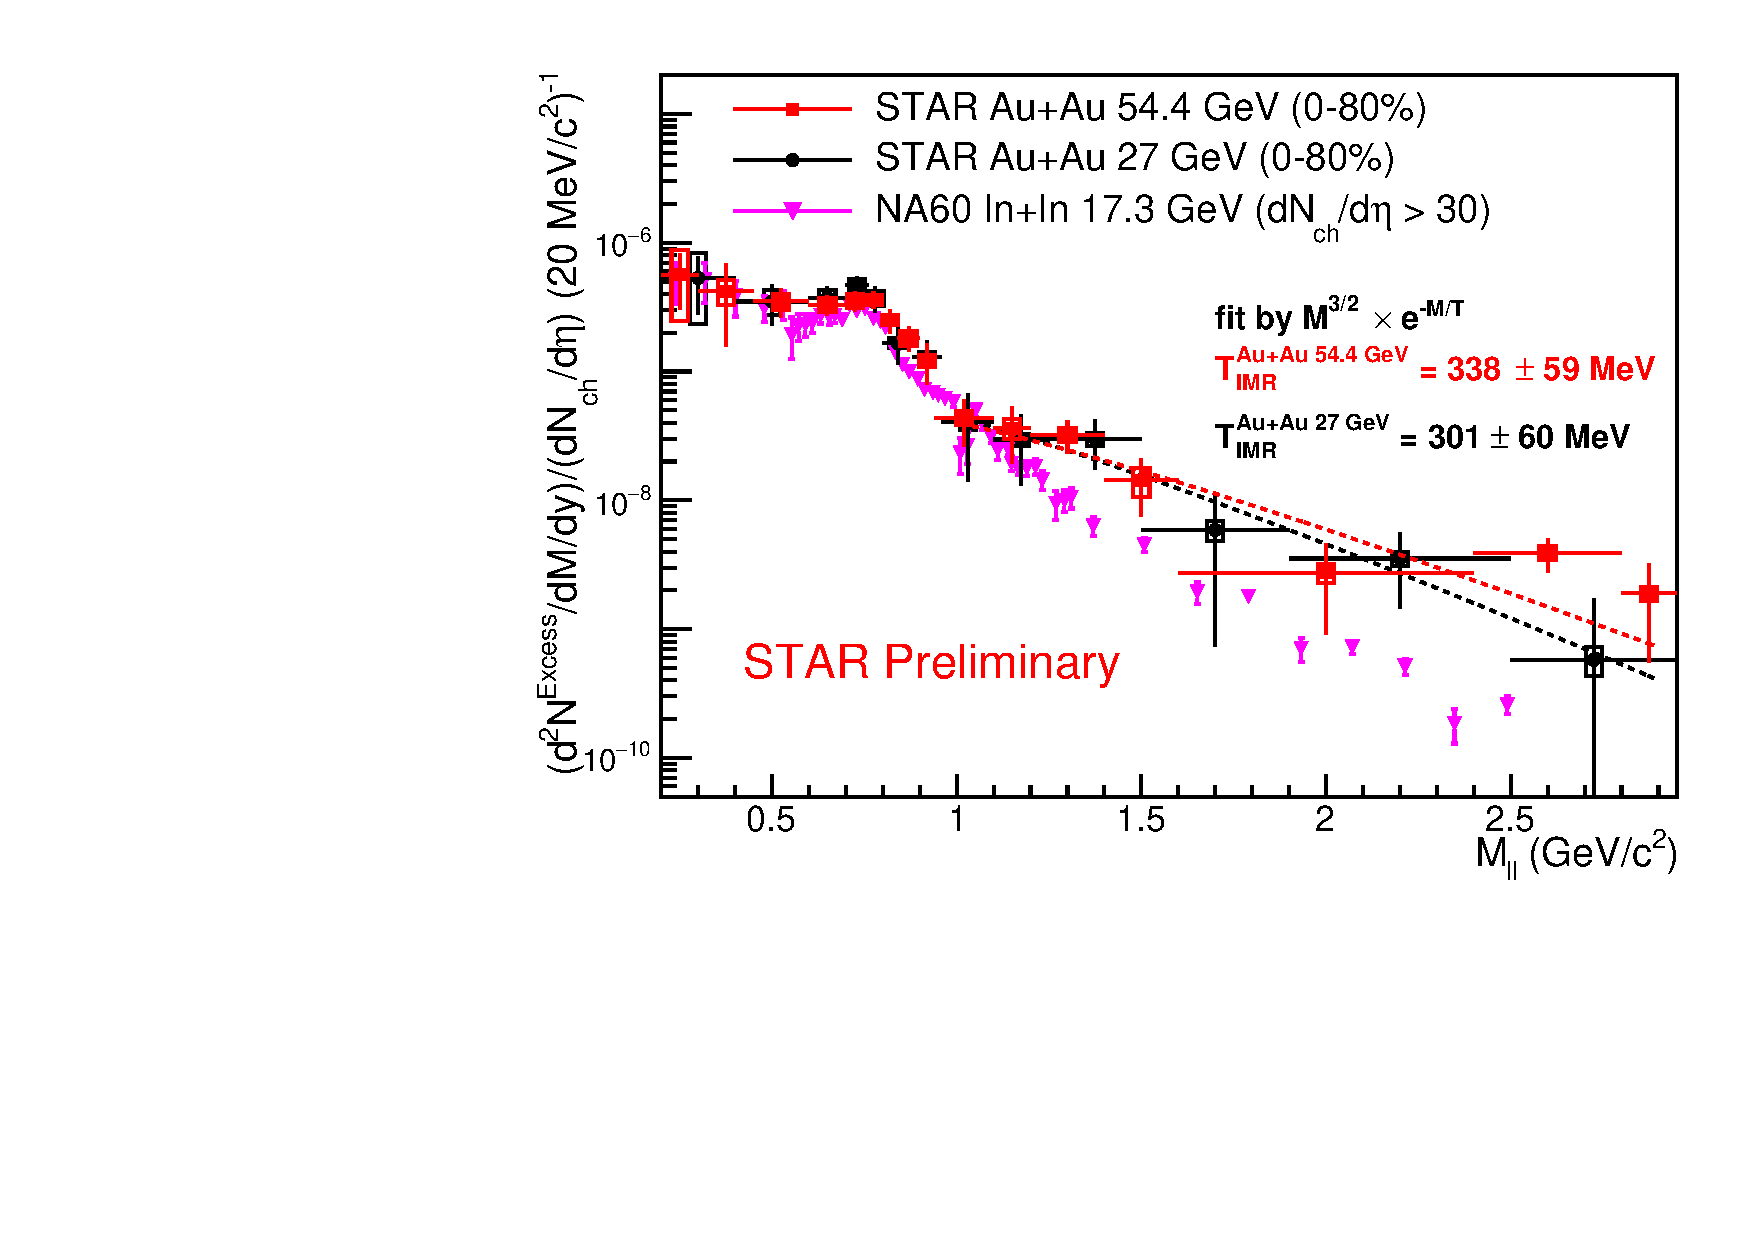
\includegraphics[width=0.75\textwidth,clip]{figures/Chapter4/Hm_ExY_FMR_54GeV_27GeV_NA60_QGPfit_icent0.pdf}
    \end{center}
    \caption[STAR实验中 \sNN = 54.4 GeV, \sNN = 27 GeV 金-金对撞以及NA60实验中\sNN = 17.3 GeV铟-铟对撞中双轻子额外产额比较示意图]{STAR实验中 \sNN = 54.4 GeV, \sNN = 27 GeV 金-金对撞以及NA60实验中\sNN = 17.3 GeV铟-铟对撞中双轻子额外产额比较示意图。在中等质量区间通过方程\ref{eq:QGP_thermal}拟合来抽取介质温度,STAR实验的抽取结果列在图中。}
    \label{fig:Hm_ExY_FMR_54GeV_27GeV_NA60_QGPfit_icent0}
\end{figure}

\begin{table}[h!]
    \centering
    \caption{54.4GeV金-金对撞中中等质量区间不同中心度通过拟合抽取得到的温度的结果}
    \label{tab:T_fitting_result_IMR}
    \begin{tabularx}{1\textwidth} {
    | >{\centering\arraybackslash}X |>{\centering\arraybackslash}X |>{\centering\arraybackslash}X |>{\centering\arraybackslash}X |>{\centering\arraybackslash}X | }
        \hline
        Centrality  & $T_{med}$ \\
        \hline
        0-80\%  & $338 \pm 58$ \\
        \hline
        0-10\%  & $371 \pm 123$ \\
        \hline
        10-40\% & $320 \pm 59$ \\
        \hline
        40-80\% & $336 \pm 55$ \\
        \hline
    \end{tabularx}
\end{table}
\section{不同中心度不同质量区间中温度抽取结果}

相比于STAR 束流能量扫描第一阶段(Beam Energy Scan Phase I, BES-I)的测量,\sNN = 54.4 GeV和 27 GeV的测量一个很大的优势就是有着更多的统计量,可以进行在不同中心度下的双电子谱的测量,基于此,在本分析当中对低质量区间和中等质量区间不同中心度下的双电子谱都进行了和前文当中相同的拟合来抽取介质的温度。

图\ref{fig:T_vs_Npart_Run17_54GeV}总结了在不同中心度下的温度抽取的结果。可以看到,在不同的中心度下相同的质量区间内的拟合结果所抽取的温度并没有明显的中心度的依赖。同时相同的质量区间内抽取的温度在不同的中心度区间也互相符合的很好。在低质量区间当中抽取的温度均在为170 MeV附近,接近理论计算中得到的夸克胶子等离子体的相变温度${\rm T_{pc} = 156 \pm 1.5 ~MeV}$。而在中等质量区间,不同中心度抽取得到的温度在各个中心度下均高于在低质量区间抽取得到的温度以及格点量子色动力学中计算得到的夸克胶子等离子体的相变温度。

\begin{figure}[htb]
    \begin{center}
    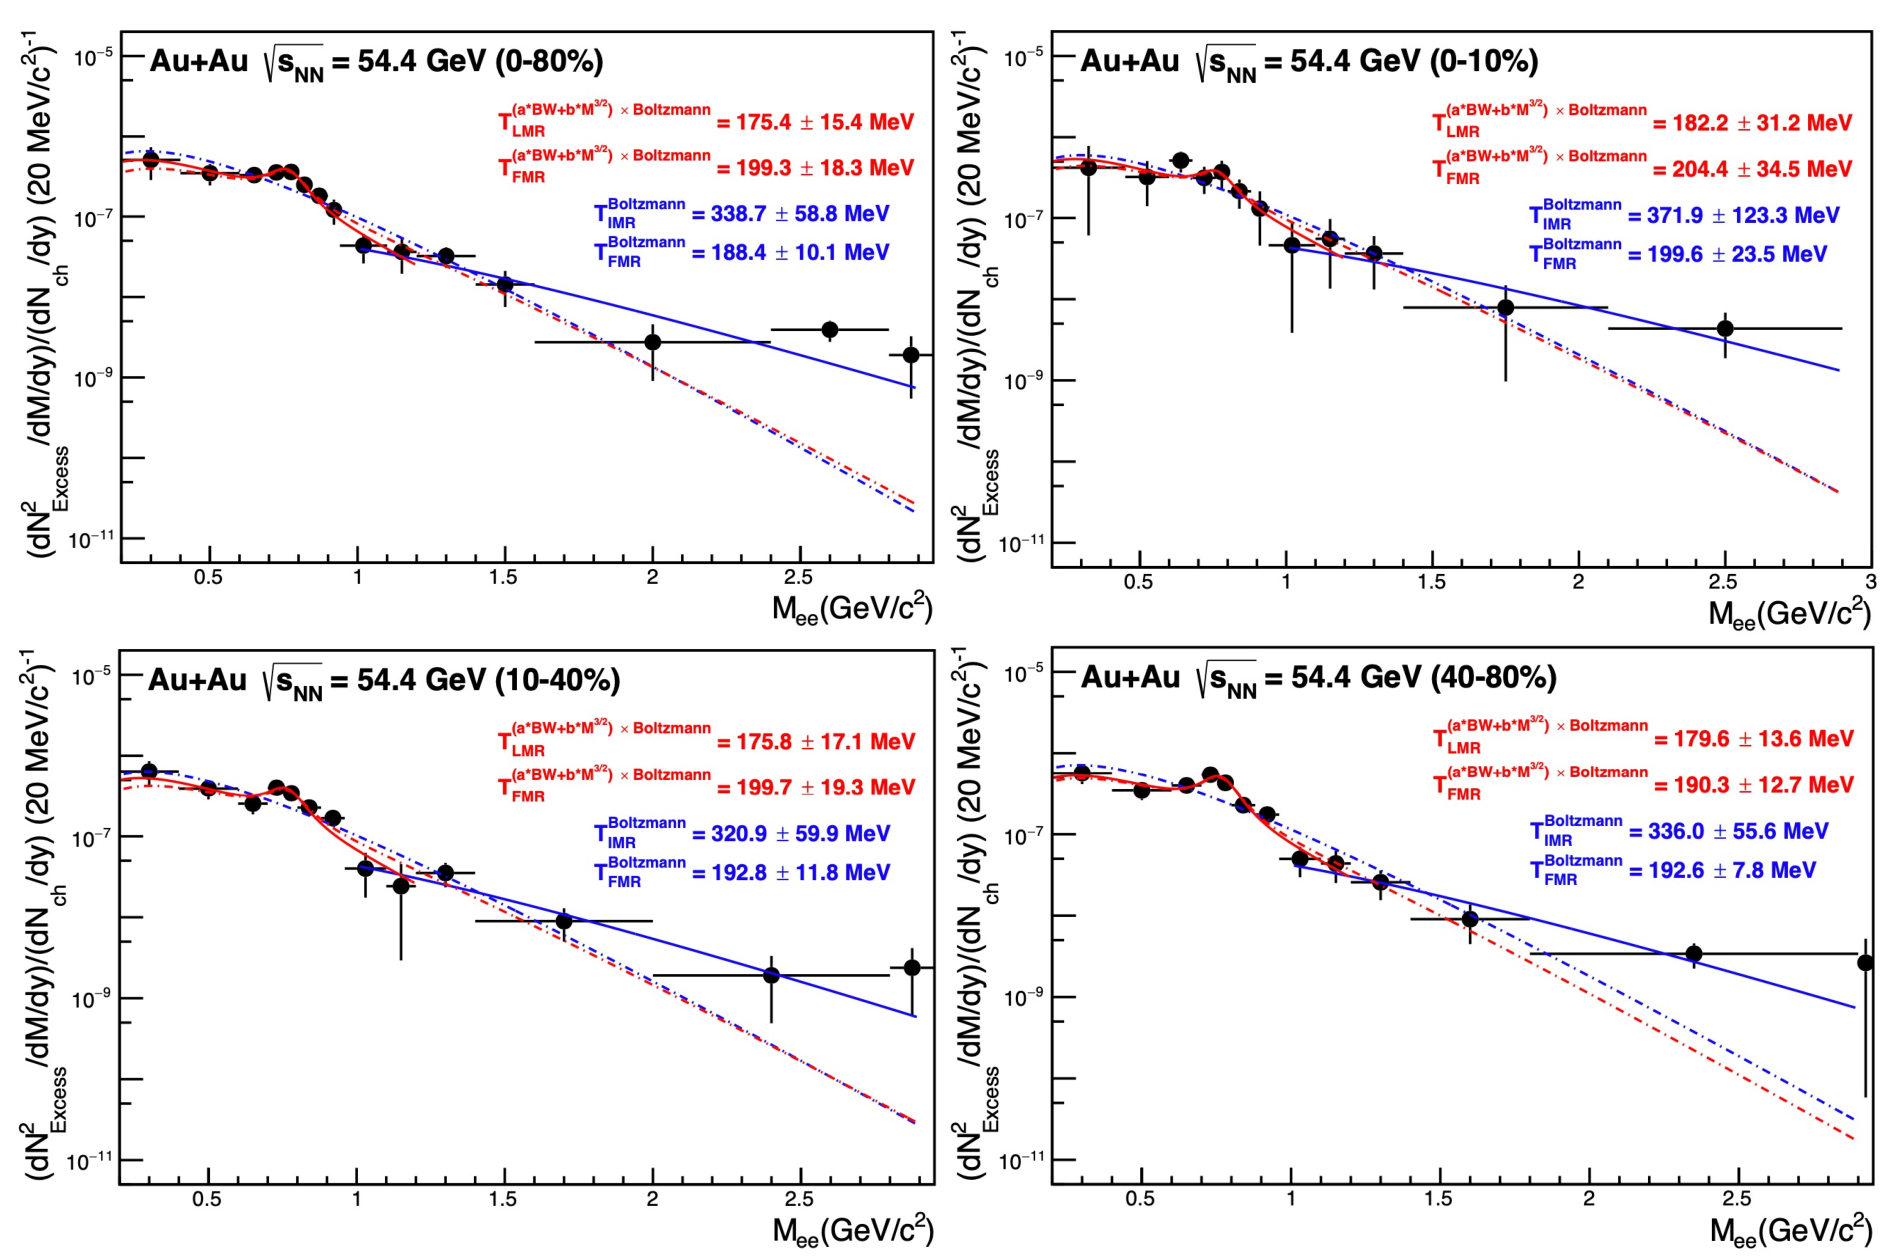
\includegraphics[width=0.75\textwidth,clip]{figures/Chapter4/Excess_fit.pdf}
    \end{center}
    \caption[\sNN = 54.4 GeV金-金对撞当中不同中心度下双电子额外产额谱及拟合结果示意图]{\sNN = 54.4 GeV金-金对撞当中不同中心度下双电子额外产额谱及拟合结果示意图,采用的拟合区间和拟合方程在图中进行标示。}
    \label{fig:Excess_fit}
\end{figure}

\begin{figure}[htb]
    \begin{center}
    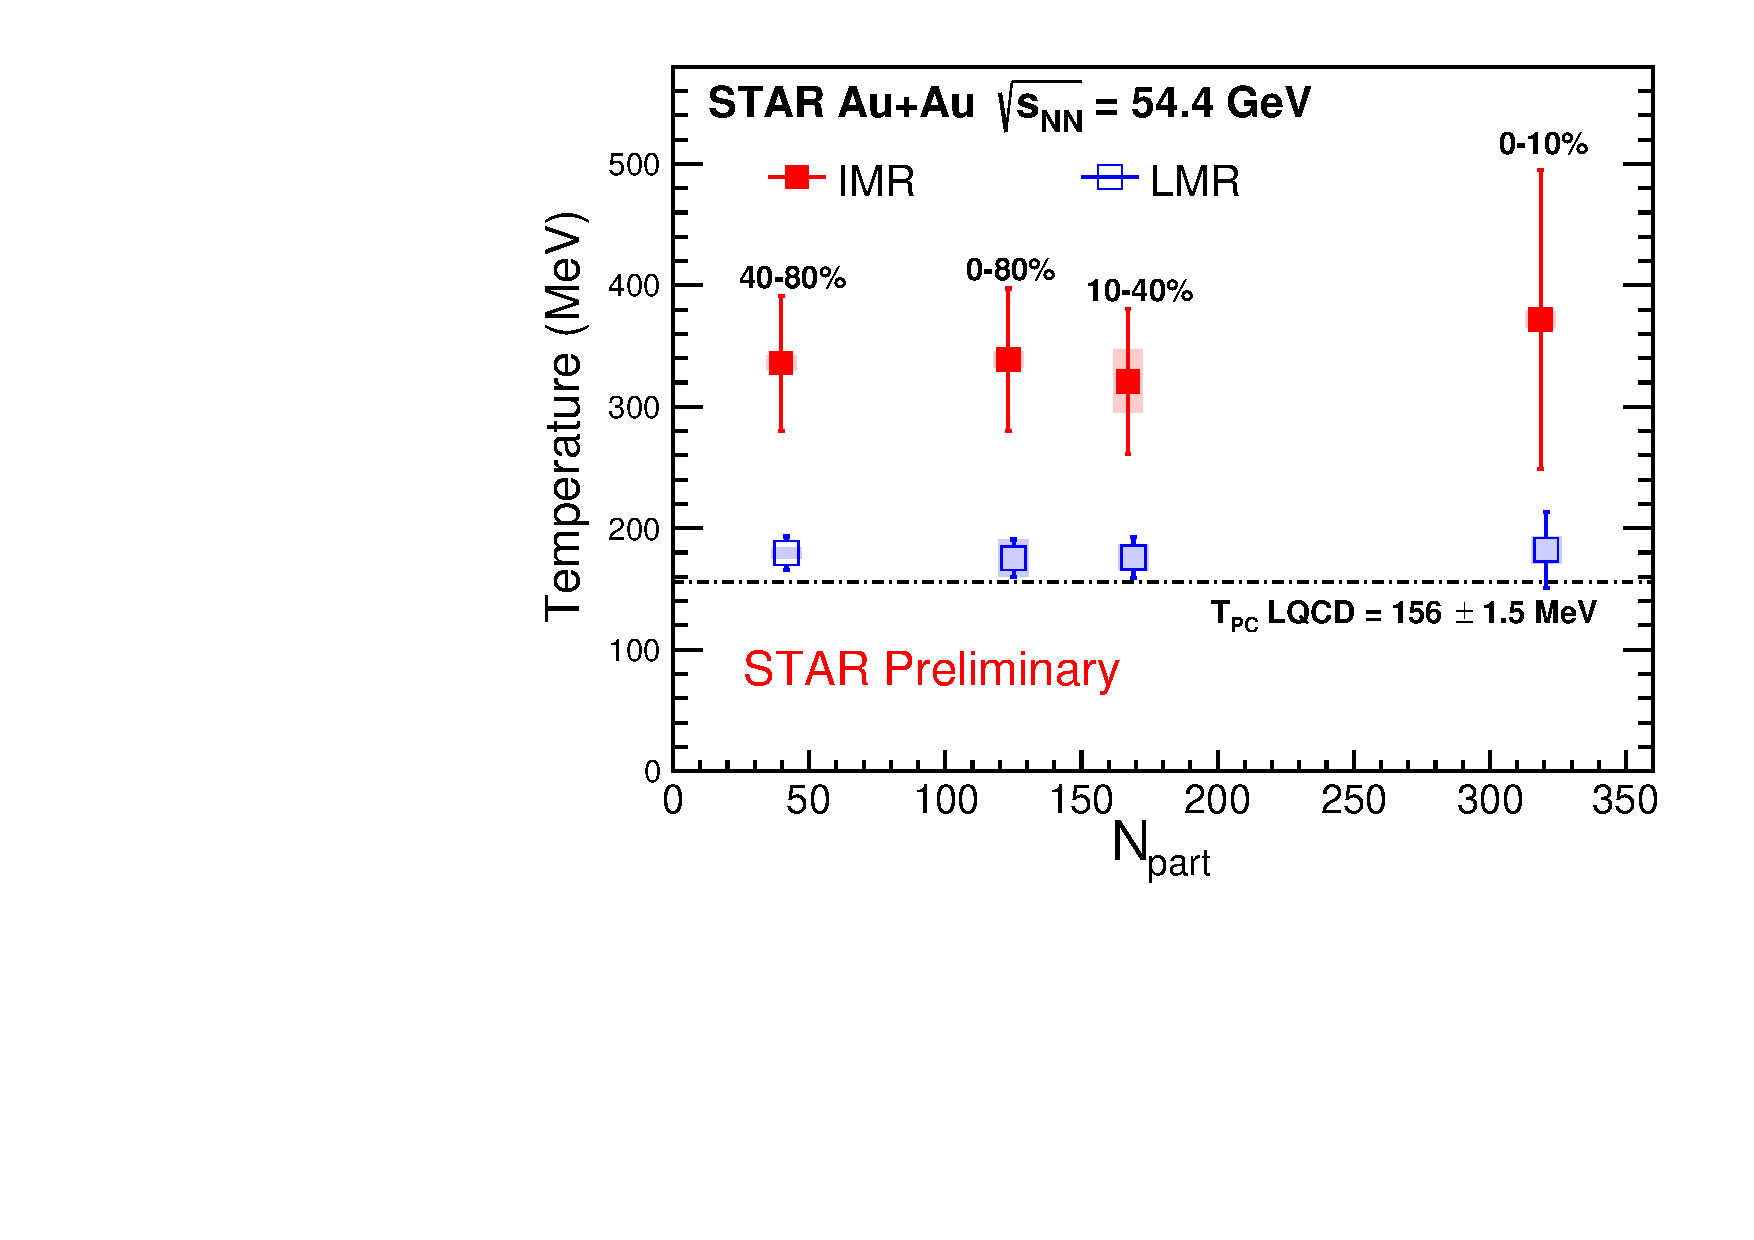
\includegraphics[width=0.75\textwidth,clip]{figures/Chapter4/T_vs_Npart_Run17_54GeV.pdf}
    \end{center}
    \caption[STAR实验中 \sNN = 54.4 GeV金-金对撞不同中心度下温度抽取比较示意图]{STAR实验中 \sNN = 54.4 GeV金-金对撞不同中心度下温度抽取比较示意图}
    \label{fig:T_vs_Npart_Run17_54GeV}
\end{figure}
\section{不同重子化学势($\mu_B$)中介质温度变化}

当对撞的束流能量发生变化时系统的重子化学势也会随之变化。在不同的对撞能量下进行温度的测量使得我们在实验上可以去探寻夸克胶子等离子体的性质。图\ref{fig:T_vs_uB_comparedNA60_HADES_phaseTransition_logx_4QM2022}为在不同的对撞能量下不同的质量区间内抽取到的介质温度随着重子化学势变化的示意图,其中包括了NA60和HADES合作组\cite{HADES:2019auv}的测量结果。在图中除了列出了格点量子色动力学计算得到的相变温度($\rm{T_PC}$)以外还列出了几种不同的统计模型(Grand-Canonical Ensemble, GCE;  Strangeness Canonical Ensemble, SCE;  Statistical Hadronization, SH\cite{STAR:2017sal,Andronic:2017pug})抽取得到的化学冻结温度($\rm{T_{ch}}$。
可以看到对RHIC以及SPS上的实验结果通过拟合低质量区间抽取得到的温度均在相变温度和化学冻结温度附近。这意味着在介质演化过程中, $\rho$主要产生在介质从解紧闭的物质相,即夸克胶子等离子体向强子物质转换的相变边界处产生。这是在首次在实验中发现可以证明这点的直接证据。

而在中等质量区间中,不同对撞能量下抽取的温度明显高于相变温度和化学冻结的温度,这再次印证了,中等质量区间内双电子的主要来源是夸克胶子等离子体的热辐射。

\begin{figure}[htb]
    \begin{center}
    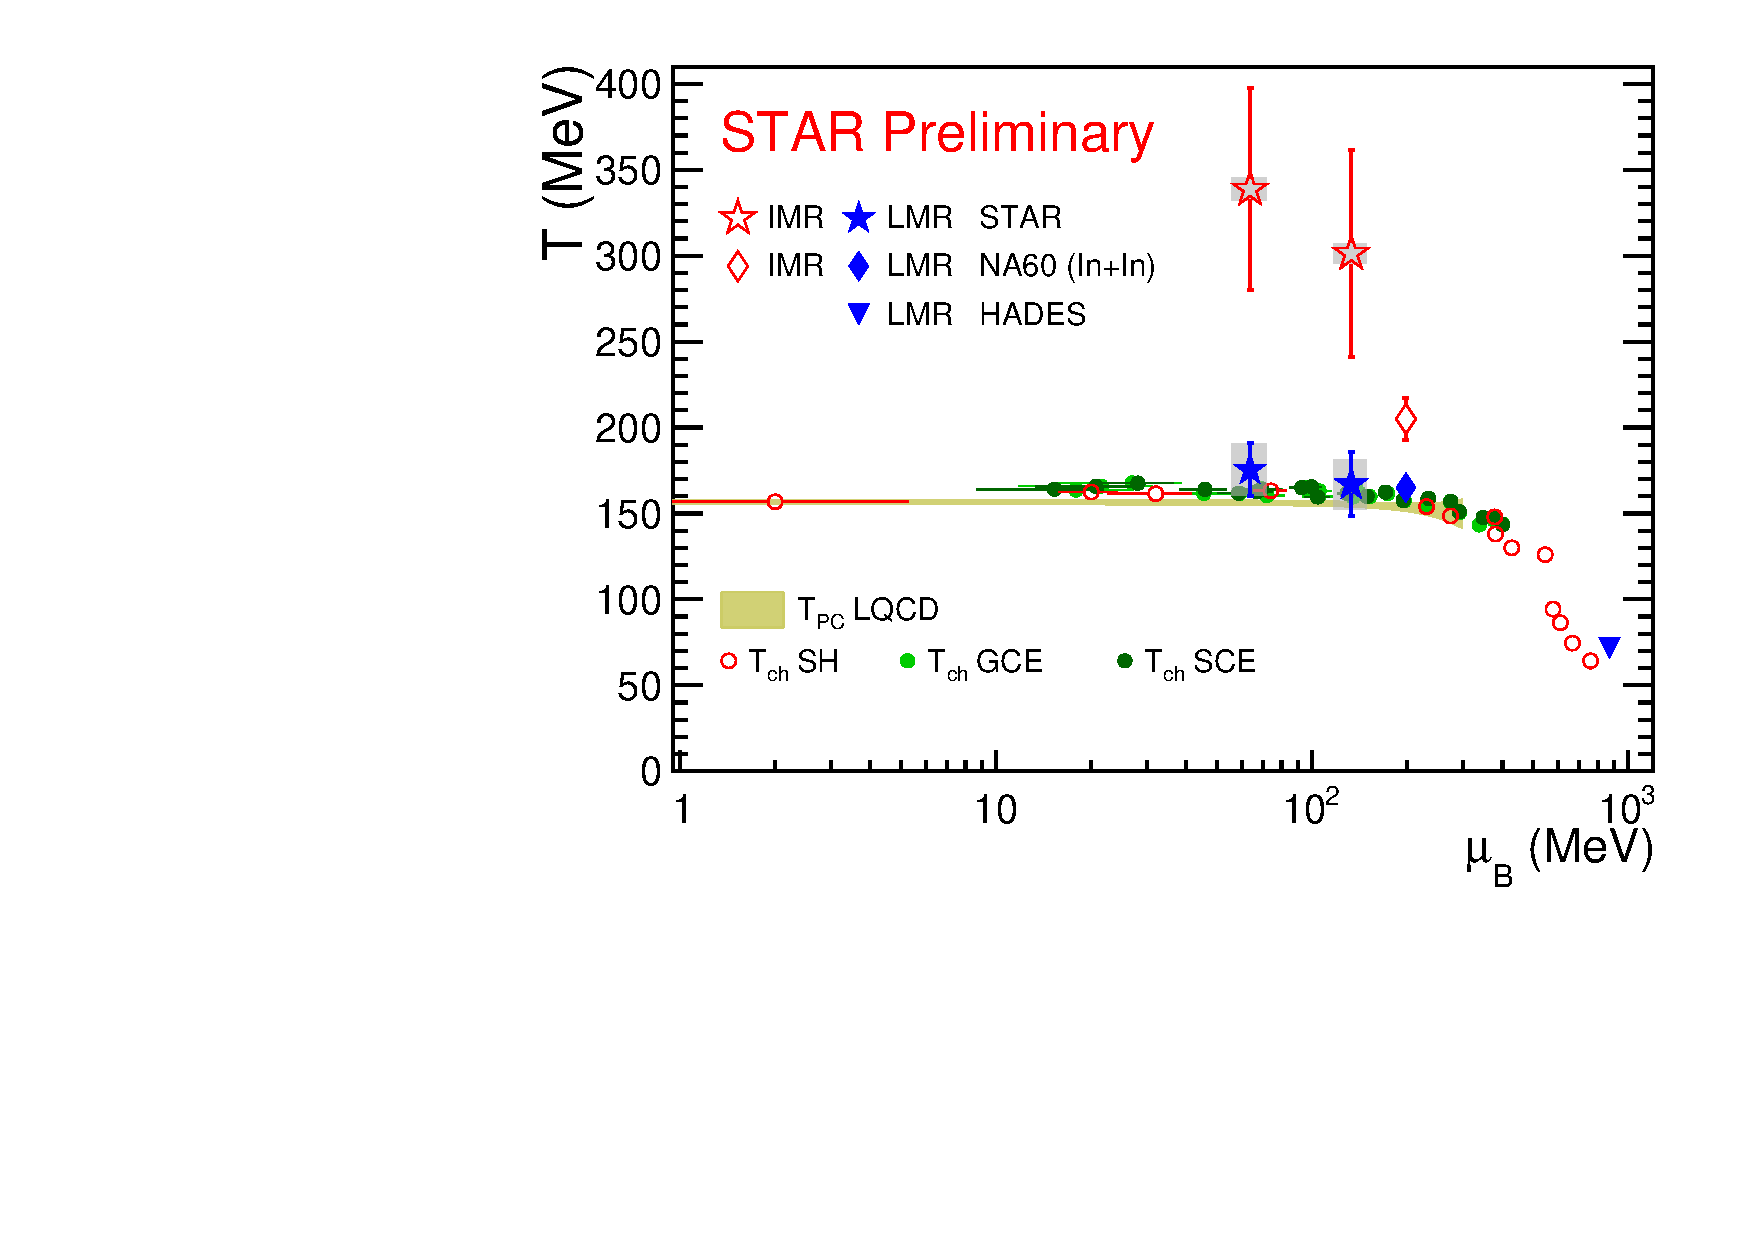
\includegraphics[width=0.75\textwidth,clip]{figures/Chapter4/T_vs_uB_comparedNA60_HADES_phaseTransition_logx_4QM2022.pdf}
    \end{center}
    \caption[双轻子额外产额谱中抽取得到的温度随重子化学势变化示意图]{双轻子额外产额谱中抽取得到的温度随重子化学势变化示意图,图中蓝色的点为在低质量区间的温度抽取结果。红色空心星形和菱形点为在中等质量区间的温度抽取结果。绿色条带为相变温度。绿色数据点和红色空心圆点为化学冻结温度。}
    \label{fig:T_vs_uB_comparedNA60_HADES_phaseTransition_logx_4QM2022}
\end{figure}